\documentclass[oneside,11pt,a4paper]{article}

% PACKAGES %

\usepackage[utf8]{inputenc}    
\usepackage[T1]{fontenc}
\usepackage[francais]{babel}
\usepackage{graphicx}
\usepackage{layout}
\usepackage{color}
\usepackage{lipsum}
\usepackage{tikz}
\usepackage{lscape}
\usepackage{listings}
\usepackage{amsmath}
\usepackage{amssymb}
\usepackage{placeins}
\usepackage{array}
\usepackage{hyperref}
\usepackage{enumerate}
%\usepackage[active,tightpage]{preview}

% D�fini les marges � 2 cm
\usepackage[top=1cm, bottom=2cm, left=2.5cm, right=2.5cm]{geometry}

% Supprime l'indentation de la premi�re ligne des paragraphes
\setlength{\parindent}{0pt}
\setlength{\parskip}{10pt}

\definecolor{keywordsColor}{rgb}{0,0.5,0}

\lstset{ %
  backgroundcolor=\color{white},   % choose the background color; you must add \usepackage{color} or \usepackage{xcolor}
  basicstyle=\footnotesize\ttfamily,        % the size of the fonts that are used for the code
  breakatwhitespace=false,         % sets if automatic breaks should only happen at whitespace
  breaklines=true,                 % sets automatic line breaking
  captionpos=none,                    % sets the caption-position to none
  columns=fixed,
  commentstyle=\color{green},    % comment style
  escapeinside={\%*}{*)},          % if you want to add LaTeX within your code
  extendedchars=true,              % lets you use non-ASCII characters; for 8-bits encodings only, does not work with UTF-8
 % frame=single,                    % adds a frame around the code
  keywordstyle=\bfseries\color{keywordsColor},       % keyword style
  language=SQL,                 % the language of the code
  numbers=left,                    % where to put the line-numbers; possible values are (none, left, right)
  numbersep=10pt,                   % how far the line-numbers are from the code
  numberstyle=\tiny\color{gray}, % the style that is used for the line-numbers
  morekeywords={REFERENCES},
  deletekeywords={YEAR},
  rulecolor=\color{black},         % if not set, the frame-color may be changed on line-breaks within not-black text (e.g. comments (green here))
  showspaces=false,                % show spaces everywhere adding particular underscores; it overrides 'showstringspaces'
  showstringspaces=false,          % underline spaces within strings only
  showtabs=false,                  % show tabs within strings adding particular underscores
  stepnumber=1,                    % the step between two line-numbers. If it's 1, each line will be numbered
  stringstyle=\color{blue},     % string literal style
  tabsize=2,                       % sets default tabsize to 2 spaces
  title=\lstname                   % show the filename of files included with \lstinputlisting; also try caption instead of title
}

% DOCUMENT %

\begin{document}
\title{Database project - deliverable 2}
\author{
	Arthur \bsc{Giroux}\\\small{205443}
	\and
	Colla \bsc{Rensch}\\\small{205814}
	\and
	Valentin \bsc{Matter}\\\small{203447}
}
\date{April $21^{\textrm{st}}$ 2013} 

\maketitle

\part*{Deliverable 1}

\section{ER model}

\begin{center}
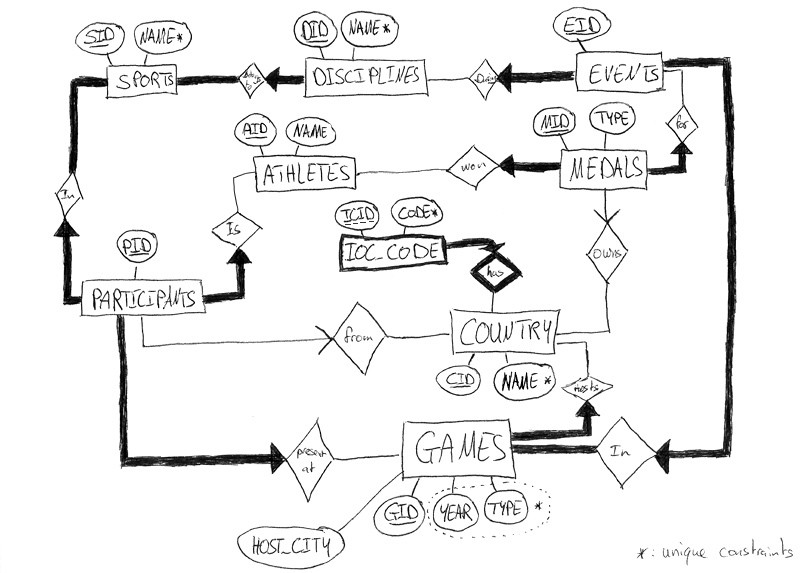
\includegraphics[height=310px]{images/ermodel.jpg}
\end{center}

\noindent\hrulefill

\section{Tables creation}

\lstinputlisting{db.sql}

\noindent\hrulefill

\section{Remarks}

\begin{itemize}
	\item Athletes is the entity that stores the information of an athlete who can then participate in multiple sports or games. Which means that if an Athlete competes twice he will have only one entry in the ATHLETES table but two in the PARTICIPANTS table.
	\item Each game should at least have one event otherwise nothing happened during he games. The same applies to sports, a sport must have at least one participant, otherwise the sport never took place during any games.
	\item Countries, sports and disciplines must have a unique name as the opposite would have no sense. For games it is the pair (YEAR,TYPE) that must be unique.
	\item Due to problem with their federations some athletes may present themselves without representing a country.
	\item Some medals could not be associated to a country as some athletes aren't as for the above point.
	\item The numbers of countries, athletes and events for a given game isn't stored in the GAMES entity as they can be easily computed using some COUNT query.
	\item The names of the events, disciplines and games are not stored as they are only the concatenation of information stored in other tables.
\end{itemize}

\noindent\hrulefill

\part*{Deliverable 2}

\section*{Modifications}

We had to slightly modify our model as we forced each athlete to have a binding participant, but we noticed that there is a quite big amount of them that do not. Therefore, we decided to slightly change our ER-model as to allow athletes to not have a binding participant. No change to the table creation code was needed as it is not possible to represent the "at least" constraint.

\noindent\hrulefill

\section*{Data import}

We chose to import the data using Java. We decided that any data that would generate a non-existent foreign key would be dropped was would any inconsistent incomplete data (i.e. medals without color)

\noindent\hrulefill

\section*{Queries}

\begin{enumerate}[A)]
	\item 
		Simple query using multiple ANDs
		\begin{lstlisting}
SELECT DISTINCT A.NAME 
FROM ATHLETES A, MEDALS M1, MEDALS M2, EVENTS E1, EVENTS E2, GAMES G1, GAMES G2
WHERE A.AID = M1.AID 
AND A.AID = M2.AID 
AND M1.MID <> M2.MID 
AND E1.EID = M1.EID 
AND E2.EID = M2.EID 
AND G1.GID = E1.GID 
AND G2.GID = E2.GID 
AND G1.TYPE <> G2.TYPE
		\end{lstlisting}
	\item 
		We have an outer-query which seeks gold medalist in sports that appear in the nested query, which computes all sports that have appeared only once
		\begin{lstlisting}
SELECT A.NAME AS ANAME, S.NAME AS SNAME
FROM SPORTS S, DISCIPLINES D, EVENTS E, ATHLETES A, MEDALS M
WHERE A.AID = M.AID 
AND M.TYPE = 'Gold' 
AND M.EID = E.EID 
AND E.DID = D.DID 
AND D.SID = S.SID 
AND S.SID IN (
	SELECT S2.SID
	FROM SPORTS S2, DISCIPLINES D2, EVENTS E2, GAMES G
	WHERE S2.SID = D2.SID 
	AND D2.DID = E2.DID 
	AND E2.GID = G.GID
	GROUP BY S2.SID
	HAVING Count(*)=1
)
ORDER BY A.NAME
		\end{lstlisting}
	\item 
		We retrieve the minimum year in which each country won its first medal using a subquery and then use a simple query to get the place hosting the corresponding games.
		\begin{lstlisting}
SELECT DISTINCT C.NAME, G.HOST_CITY
FROM COUNTRIES C, MEDALS M, EVENTS E, GAMES G, (
	SELECT C2.CID, MIN( G2.YEAR ) AS MIN_YEAR
	FROM COUNTRIES C2, MEDALS M2, EVENTS E2, GAMES G2
	WHERE C2.CID = M2.CID
	AND M2.EID = E2.EID
	AND E2.GID = G2.GID
	GROUP BY C2.CID
) TMP
WHERE C.CID = M.CID
AND M.EID = E.EID
AND E.GID = G.GID
AND C.CID = TMP.CID
AND G.YEAR = TMP.MIN_YEAR
ORDER BY C.NAME
		\end{lstlisting}
	\item 
		We unite (UNION) two same queries using "Summer" for one and "Winter" for the other and compute the number of medals for each country given the type (Summer or Winter), we then order them despondingly and limit the table to 1
		\begin{lstlisting}
(
	SELECT COUNT(M.CID) AS MAXIMUM, C.NAME, G.TYPE
	FROM COUNTRIES C, GAMES G, EVENTS E, MEDALS M
	WHERE C.CID = M.CID 
	AND M.EID = E.EID 
	AND E.GID = G.GID 
	AND G.TYPE = 'Summer'
	GROUP BY C.NAME 
	ORDER BY MAXIMUM DESC 
	LIMIT 1
) UNION (
	SELECT COUNT(M.CID) AS MAXIMUM, C.NAME, G.TYPE
	FROM COUNTRIES C, GAMES G, EVENTS E, MEDALS M
	WHERE C.CID = M.CID 
	AND M.EID = E.EID 
	AND E.GID = G.GID 
	AND G.TYPE = 'Winter'
	GROUP BY C.NAME 
	ORDER BY MAXIMUM DESC 
	LIMIT 1
)
		\end{lstlisting}
	\item 
		Simple GROUP BY + HAVING query
		\begin{lstlisting}
SELECT G.HOST_CITY
FROM GAMES G
GROUP BY G.HOST_CITY
HAVING COUNT(*) > 1
ORDER BY G.HOST_CITY
		\end{lstlisting}
	\item 
		We use two table of participants and two tables for countries and then just use ANDs to make find the athletes that competed for at least two countries
		\begin{lstlisting}
SELECT DISTINCT(A.NAME)
FROM ATHLETES A, PARTICIPANTS P1, PARTICIPANTS P2, COUNTRIES C1, COUNTRIES C2
WHERE A.AID = P1.AID 
AND A.AID = P2.AID 
AND P1.PID <> P2.PID 
AND P1.CID = C1.CID 
AND P2.CID = C2.CID 
AND C1.CID <> C2.CID
ORDER BY A.NAME
		\end{lstlisting}
	\item 
		The subquery computes the participants count for each country for a particular games. Then, for each game, the outer-query finds the countries having a participants count greater than all the results of the subquery.
		\begin{lstlisting}
SELECT G.YEAR, G.TYPE, C.NAME, COUNT(*) AS COUNT 
FROM COUNTRIES C, PARTICIPANTS P, GAMES G 
WHERE G.GID = P.GID AND C.CID=P.CID 
GROUP BY P.GID, P.CID 
HAVING COUNT(*) >= ALL (
	SELECT COUNT(*) 
	FROM PARTICIPANTS P2 
	WHERE P.GID=P2.GID 
	GROUP BY P2.GID, P2.CID
)
ORDER BY G.YEAR
		\end{lstlisting}
	\item 
		We simply take the COUNTRIES and use a nested query to delete all entries that do not appear in the MEDALS table
		\begin{lstlisting}
SELECT DISTINCT C.NAME
FROM COUNTRIES C
WHERE C.CID NOT IN (
	SELECT M.CID
	FROM MEDALS M
	WHERE M.CID IS NOT NULL
)
		\end{lstlisting}
\end{enumerate}

\noindent\hrulefill

\section*{Front-end}

Our web front-end is available at \url{http://db.tamere.ch/}. It was made using PHP and MySQL.

\begin{center}
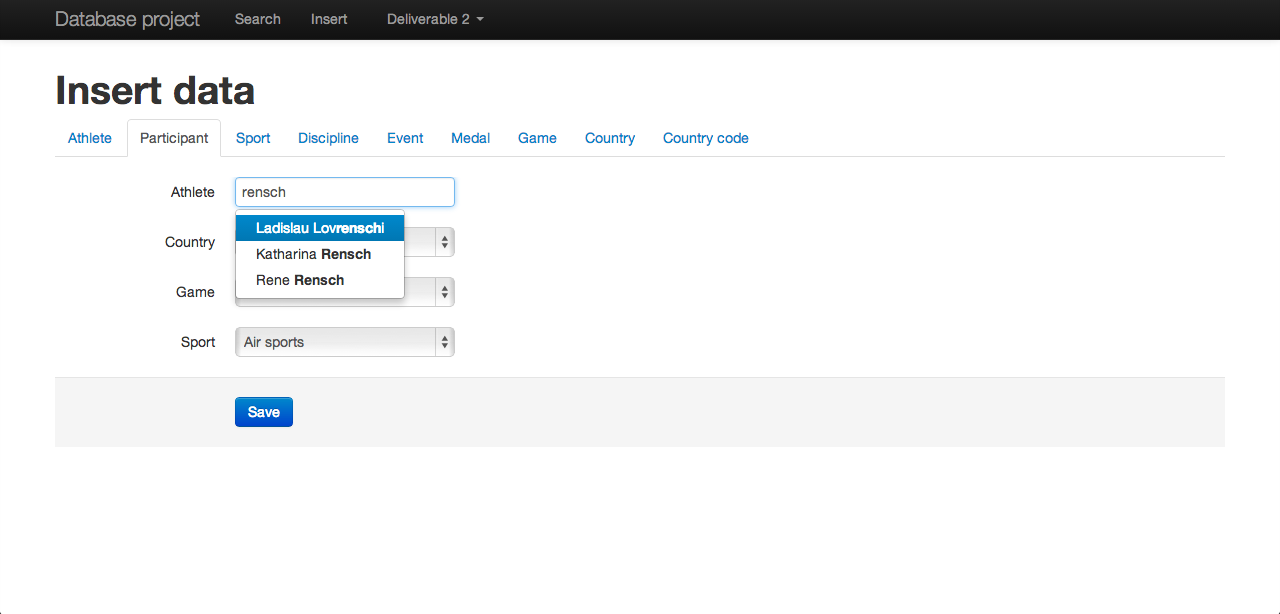
\includegraphics[height=210px]{images/capt1.png}
The insertion page
\end{center}

\begin{center}
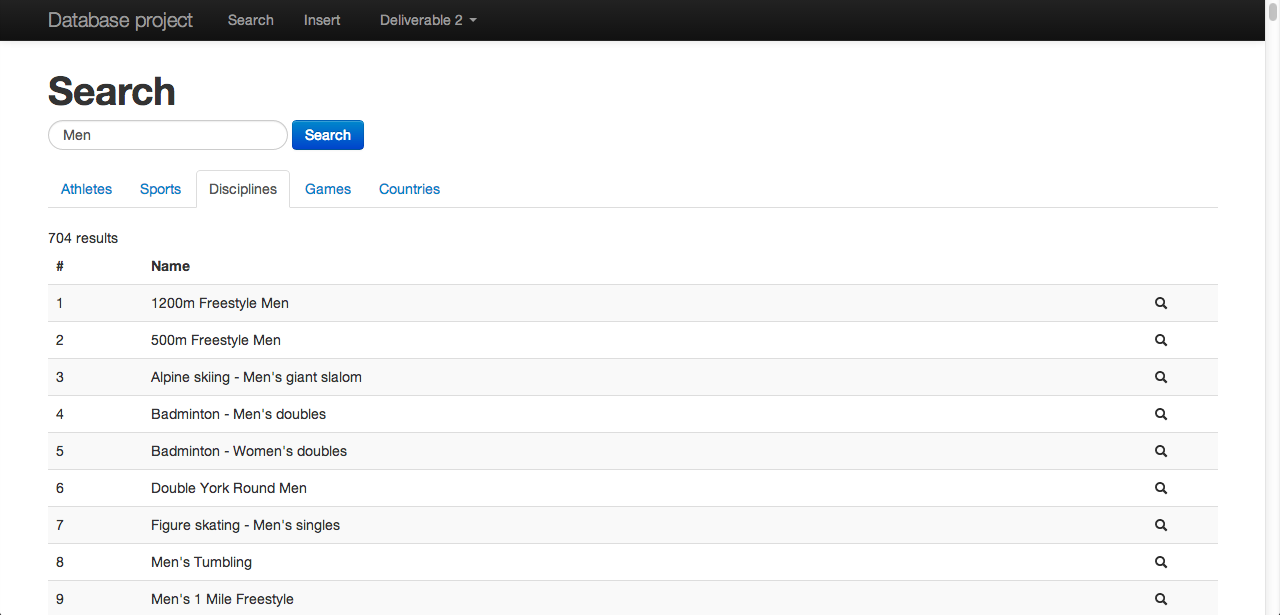
\includegraphics[height=210px]{images/capt2.png}
The search page
\end{center}

\begin{center}
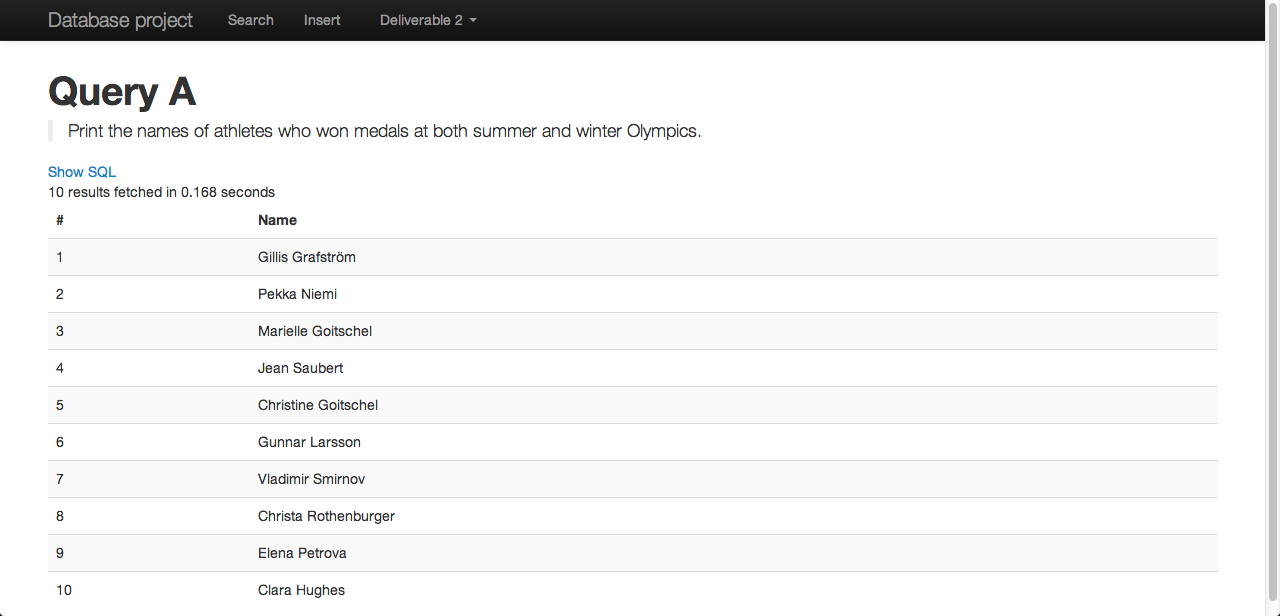
\includegraphics[height=210px]{images/capt3.png}
The result of one of the queries
\end{center}

\noindent\hrulefill

\part*{Deliverable 3}

- CASCADE CASCADE CASCADE EVERYWHERE !!

- Add TID

-this shit :
\begin{lstlisting}
CREATE VIEW MEDALS_UNIQUE AS (
  SELECT MIN(M.MID) AS MID, M.CID, M.TYPE, M.EID 
  FROM MEDALS M
  WHERE M.TID IS NOT NULL
  GROUP BY M.TID
) UNION (
  SELECT M.MID, M.CID, M.TYPE, M.EID 
  FROM MEDALS M
  WHERE M.TID IS NULL
)
\end{lstlisting}

\end{document}